%
% system_overview.tex
%
% Copyright The EPS 2.0 Contributors.
%
% EPS 2.0 Documentation
%
% This work is licensed under the Creative Commons Attribution-ShareAlike 4.0
% International License. To view a copy of this license,
% visit http://creativecommons.org/licenses/by-sa/4.0/.
%

%
% \brief System overview chapter.
%
% \author Gabriel Mariano Marcelino <gabriel.mm8@gmail.com>
% \author Yan Castro de Azeredo <yan.ufsceel@gmail.com>
%
% \version 0.3.0
%
% \date 2021/02/10
%

\chapter{System Overview} \label{ch:system-overview}

The board has a MSP430 low-power MCU\nomenclature{\textbf{MCU}}{\textit{Microcontroller.}} that runs the firmware application intended to control and comunicate with its peripherals, subsystems and other modules. The programming language used is C and the firmware was developed using the Code Composer Studio IDE\nomenclature{\textbf{IDE}}{\textit{Integrated Development Environment.}} (a.k.a. CCS) for compiling, programming and testing. The module has many tasks, such as interfacing internal peripherals and communicating with other boards, over distinct protocols and time requirements. 
Then, in order to improve predictability, a Real Time Operating System (RTOS\nomenclature{\textbf{RTOS}}{\textit{Real Time Operating System.}}) is used to ensure that the deadlines are observed, even under a fault situation in a routine. The RTOS chosen is the FreeRTOS (v10.2.1), since it is designed for embedded systems applications and it was already validated in space applications. The firmware architecture follows an abstraction layer scheme to facilitate higher level implementations and allow more portability across different hardware platforms, see \autoref{sec:system-layers} for more details.

The EPS 2.0 is compatible with GOMspace Solar Panels or with panels of similar characteristics. Algorithms are implemented for MPPT improving power generation, also through measurements the load output can be regulated for a more efficient power distribution to the nanosattelite.

\section{Product tree}

The product tree of the EPS 2.0 module is available in \autoref{fig:product-tree}.

\begin{figure}[!ht]
    \begin{center}
        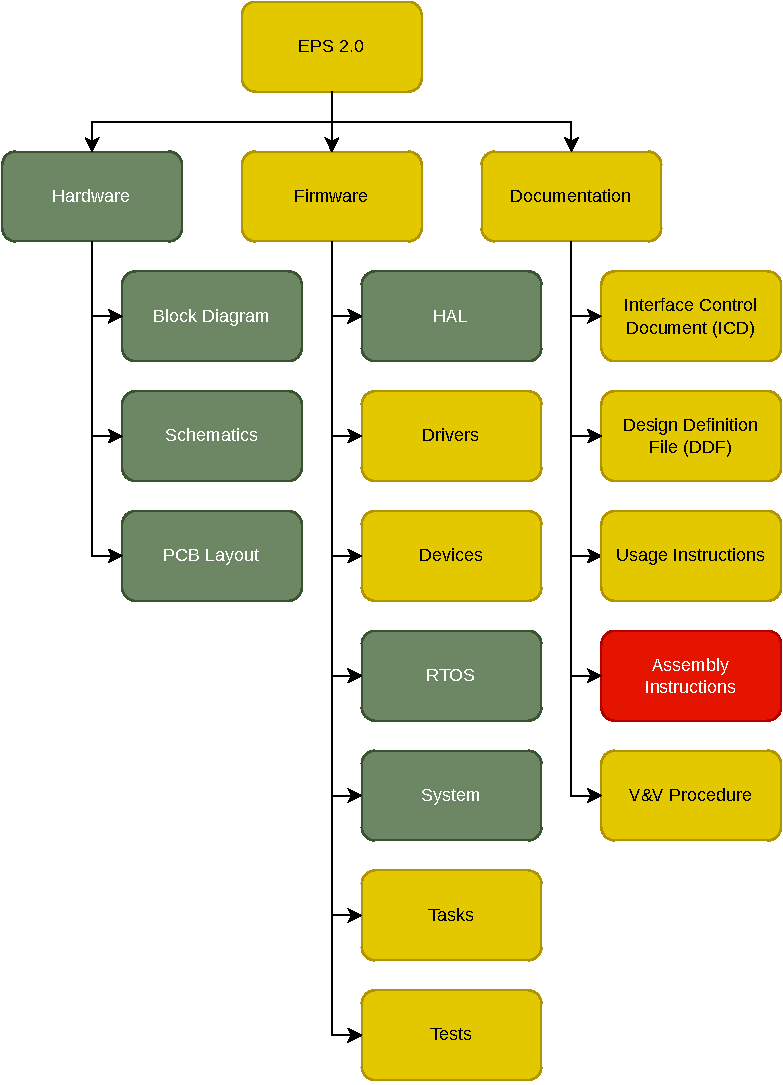
\includegraphics[width=0.8\textwidth]{figures/product-tree.pdf}
        \caption{Product tree of the EPS 2.0 module.}
        \label{fig:product-tree}
    \end{center}
\end{figure}

\section{MCU Block Diagram}

The \autoref{fig:mcu-block-diagram} presents a simplified view of the module subsystems and interfaces though the microcontroller perspective. 
The MCU has a programming JTAG\nomenclature{\textbf{JTAG}}{\textit{Joint Test Action Group.}}, a dedicated UART\nomenclature{\textbf{UART}}{\textit{Universal Asynchronous Receiver/Transmitter.}} debug interface and 4 communication buses, divided in 4 different protocols (I2C\nomenclature{\textbf{I2C}}{\textit{Inter-Integrated Circuit.}}, SPI\nomenclature{\textbf{SPI}}{\textit{Serial Peripheral Interface.}} and UART). 

There is a I2C buffer to allow secure and proper communication with the OBDH 2.0 module \cite{obdh2}.
The SPI protocol is used for controling and retriving data from a additional ADC\nomenclature{\textbf{ADC}}{\textit{Analog-to-Digital Converter.}} IC that measures temperature sensors (RTDs\nomenclature{\textbf{RTD}}{\textit{Resistance Temperature Detector.}}) on the batteries board and solar panels.
The I2C protocol measures several parameters from the Batteries Managment Subsystem and sends them to the EPS 2.0 MCU.
The UART bus that goes to the PC/104 is used for basic telemetry to be sent to the beacon microcontroller within the TTC module.
Besides this channels, there are GPIO\nomenclature{\textbf{GPIO}}{\textit{General Purpose Input/Output.}} connections for enabling and disabling power buses, for hard code PCB versioning and some optional GPIOs that can be added and used though the PC/104 interface. 

The MCU makes meassuments of current and voltage of the solar panels from its ADC ports for the MPPT Subsystem, also from this data the MPPT is controled by the microcontroller through PWM\nomenclature{\textbf{PWM}}{\textit{Pulse Width Modulation.}} signals.

A external charger is used for charging the batteries and kill-switches for powering off the EPS 2.0 module during test phase, for flight the kill-switches are also connected to the button switches present on a CubeSat structure.   

\begin{figure}[!ht]
    \begin{center}
        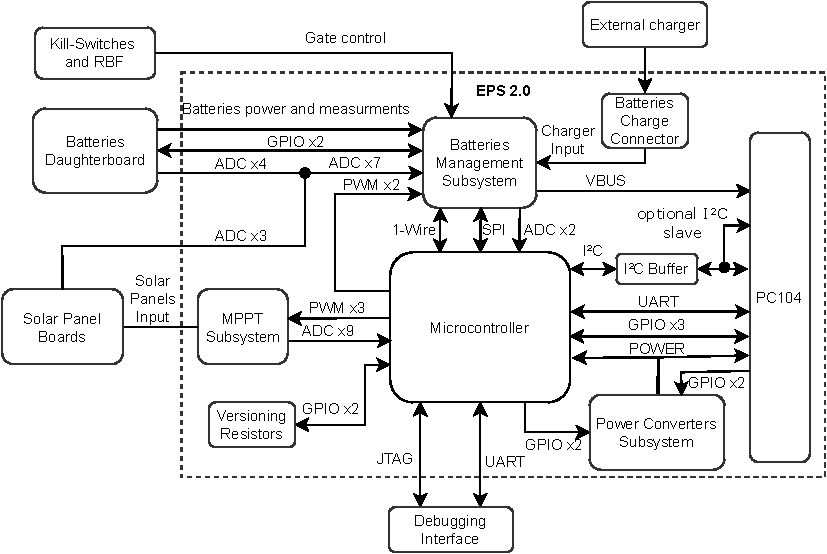
\includegraphics[width=0.75\textwidth]{figures/eps2_mcu_diagram.pdf}
        \caption{EPS 2.0 MCU Block diagram.}
        \label{fig:mcu-block-diagram}
    \end{center}
\end{figure}

\section{Power Block Diagram}

The \autoref{fig:power-block-diagram} presents a more detailed view of the power subsystems that complements the MCU Block Diagram. More details and descriptions about these hardware components and interfaces are provided in the \autoref{ch:hardware}.

\begin{figure}[!ht]
    \begin{center}
        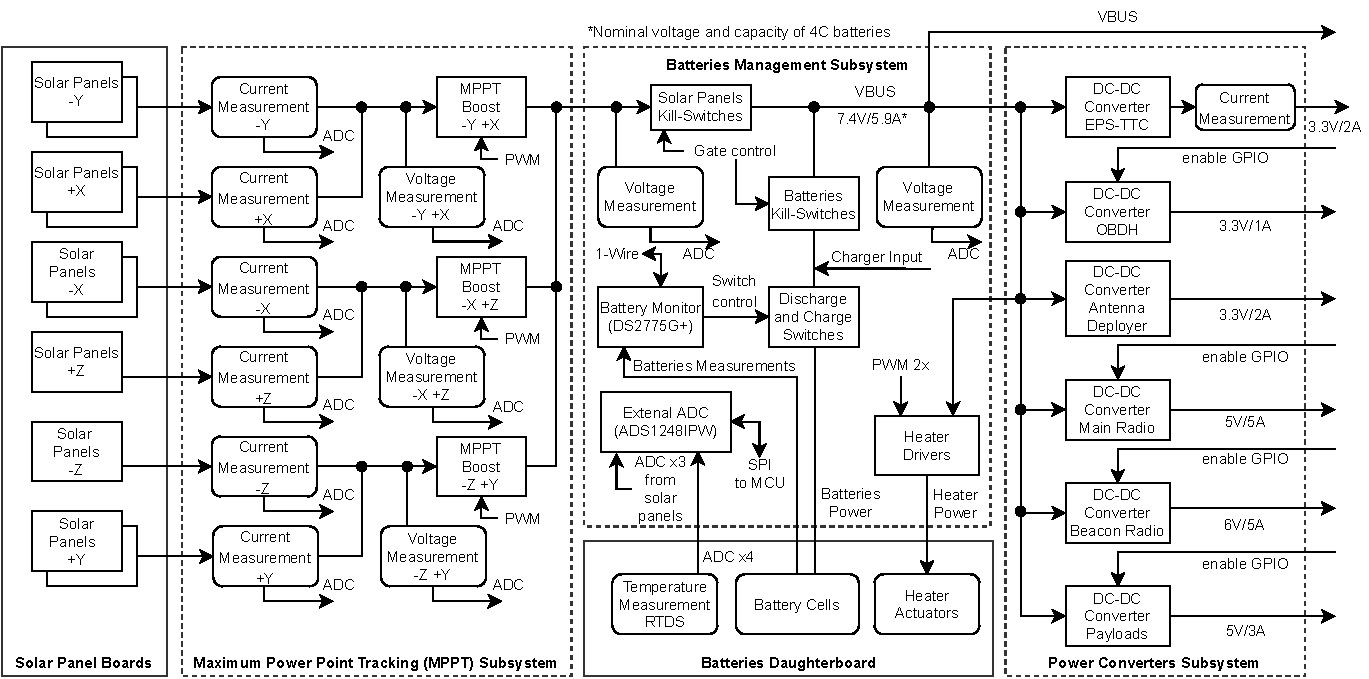
\includegraphics[width=\textwidth]{figures/eps2_power_diagram.pdf}
        \caption{EPS 2.0 Power Block diagram.}
        \label{fig:power-block-diagram}
    \end{center}
\end{figure}

\section{System Layers} \label{sec:system-layers}

As herein mentioned, the system is divided in various abstraction layers to favor high level firmware implementations. The \autoref{fig:system-layers} shows this scheme, which is composed of third-part drivers at the lowest layer above the hardware, the operating system as the base building block of the module, the devices handling implementation, and the application tasks in the highest layer. More details are provided in the \autoref{ch:firmware}.

\begin{figure}[!ht]
    \begin{center}
        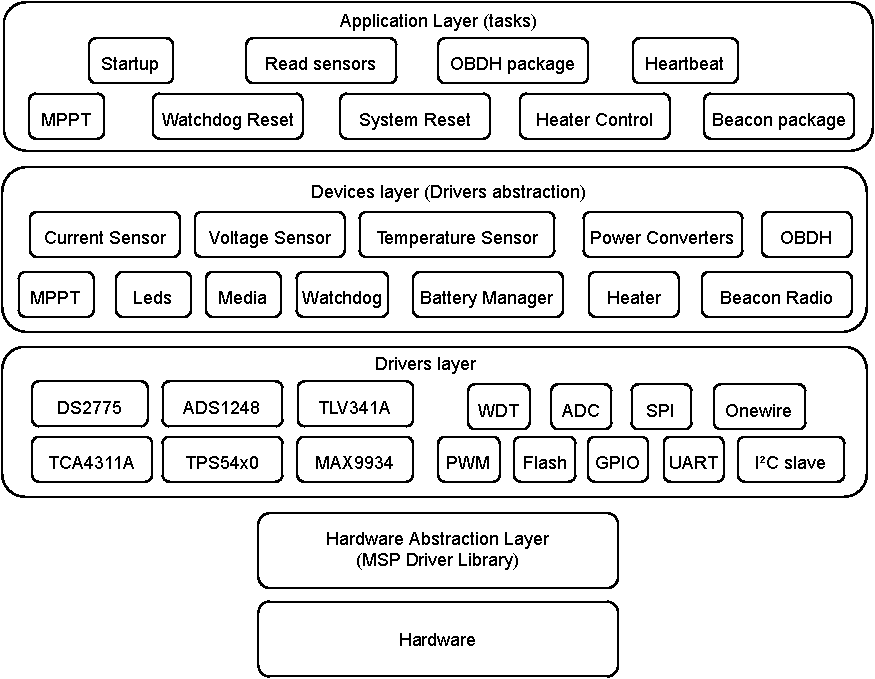
\includegraphics[width=0.75\textwidth]{figures/eps-system-layers.pdf}
        \caption{System layers.}
        \label{fig:system-layers}
    \end{center}
\end{figure}

\section{Operation} \label{sec:operation}

The system operates through the sequencial execution of routines (tasks in the context of the operating system) that are scheduled and multiplexed along the time. Each routine has a priority and a periodicity, which determine the following execution, the set of functionalities currentely running, and the memory usage management. Besides this deterministic scheduling system, the routines have communication channels with each other through the usage of queues, which provides a robust synchorization scheme. In the \autoref{ch:firmware} the system operation and the internal nuances are described in detail. Then, this section use a top view user perspective to describe the module operation.

\subsection{Execution Flow}
% Add here a diagram showing a simple flowchart or use cases to represent how the EPS works.

\subsection{Data Flow}
% Add here a flowchart or diagram showing where and how the data is generated and transfered across diferent modules and peripherals.

\subsection{Status LEDs} \label{status-leds}

On the development version of the board, there are ten LED\nomenclature{\textbf{LED}}{\textit{Light-Emitting Diode.}}s that indicates some behaviours of the systems. This set of LEDs can be seen on \autoref{fig:status-leds}.

\begin{figure}[!ht]
    \begin{center}
        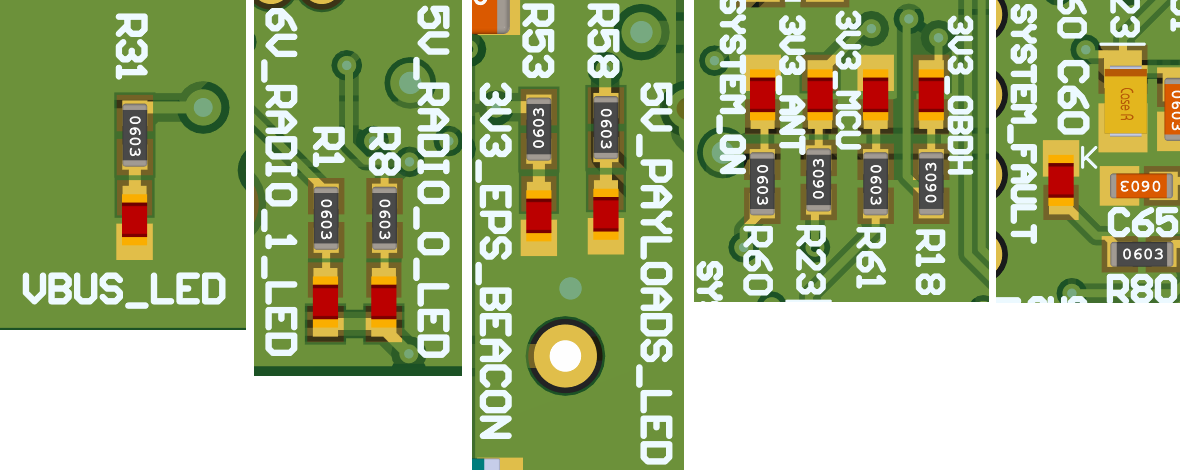
\includegraphics[width=\textwidth]{figures/status_leds.png}
        \caption{Available status LEDs.}
        \label{fig:status-leds}
    \end{center}
\end{figure}

A description of each of these LEDs are available below:

\begin{itemize}
    \item \textbf{6V\_RADIO\_1\_LED}: Indicates that the radio 1 transceiver 6V power is being sourced.
    \item \textbf{5V\_RADIO\_0\_LED}: Indicates that the radio 0 transceiver 5V power is being sourced.
    \item \textbf{SYSTEM\_ON}: Heartbeat of the system. Blinks at a frequency of 1 Hz when the system is running properly.
    \item \textbf{SYSTEM\_FAULT}: Indicates an error has occurred during the running firmware of the board.
    \item \textbf{3V3\_ANT}: Indicates that the antenna deployer 3.3V power is being sourced.
    \item \textbf{3V3\_MCU}: Indicates that the EPS2 MCU 3.3V power is being sourced.
    \item \textbf{3V3\_OBDH}: Indicates that the OBDH module 3.3V power is being sourced.
    \item \textbf{3V3\_EPS\_BEACON}: Indicates that the EPS2 board and beacon MCU 3.3V power is being sourced.
    \item \textbf{5V\_PAYLOADS\_LEDS}: Indicates that the payloads 5V power is being sourced.
    \item \textbf{VBUS\_LED}: Indicates that the main power bus from the batteries is being sourced.
\end{itemize}

These LEDs are not mounted in the flight version of the module.

\section{Hard Code Versioning}

On the EPS2 board there are 2 GPIOs dedicated for hard code versioning.
The on-board firmware can read these pins to indentify the correct version of the hardware project.
Each line can be either pulled to VCC or ground, representing in binary as 1 and 0 respectively.
The \autoref{tab:versioning-resistors} shows the representation of the versioning up to the latest revision of the project.

\begin{table}[!h]
    \centering
    \begin{tabular}{lcc}
        \toprule[1.5pt]
        \textbf{Version}    &   \textbf{P3.5 (pin code) / 47 (pin number)}    &    \textbf{P3.4 (pin code) / 46 (pin number)}\\
        \midrule
        v0.1                & 0                 & 0              \\
        v0.2                & 0                 & 1              \\
        \bottomrule[1.5pt]
    \end{tabular}
    \caption{Hard code versioning table.}
    \label{tab:versioning-resistors}
\end{table}
